\label{current_research}
Supporting a diverse set of computational campaigns on HPC resources requires the used middleware to be able to support workflows with different computational characteristics.
Scientific applications that are compute-intensive are very well supported by HPC resources.
On the other hand, data-intensive applications do not have the same level of support.
A computational campaign can be comprised by workflows that can be compute or data intensive.
As a result, supporting both types of workflows on HPC resources is important.

\subsection{Data analytics on HPC}
\label{data_analysis_hpc}
Task-parallel frameworks, used mainly for data-intensive applications, involve partitioning a workload into a set of self-contained units of work. 
Based on the application, these tasks can be independent or coupled with varying degrees of data dependencies. 
Scientific workflows exploit task parallelism for simulations as well as data analysis.
Scientific data analysis tools, such as MDAnalysis~\cite{gowers2016mdanalysis,michaud2011mdanalysis}, support domain specific data analytics, but scaling on large data volumes remains a challenge.
These volumes of data are either produced on HPC resources via simulations or acquired via sensors on HPC resources.
As a result, there is a need to support scalable data analytics on the same resources, and especially on HPC resources.

Task-parallel frameworks such as Hadoop~\cite{hadoop}, and Spark~\cite{zaharia2010spark} have been used widely to support scalable data analytics.
There are frameworks for executing and running Hadoop and Spark on HPC resources.
Framework, such as MagPie~\cite{magpie}, JUMMP~\cite{moody2013jummp}, and MyHadoop~\cite{krishnan04myhadoop}, support Hadoop on HPC resources.
These approaches do not support the interoperability of data generation/ acquisition and data analysis that is required.

The Pilot-abstraction~\cite{luckow2012pstar} has been successfully used on HPC resources to support a diverse set of task-parallel applications, via its implementation RADICAL-Pilot~\cite{merzky2019using}.
We extended RADICAL-Pilot to support data-parallel frameworks, such as Hadoop and Spark, on HPC resources~\cite{luckow2016hadoop}.
The extension allows users to execute Hadoop- or Spark-style data analysis on HPC resources.
It is important to note that RADICAL-Pilot is responsible to start, and manage a Hadoop or Spark cluster seamlessly from the user.

We investigated~\cite{paraskevakos2018task} the suitability of task-parallel frameworks for Molecular Dynamics trajectory data analysis. 
The analysis included Spark~\cite{zaharia2010spark}, Dask~\cite{rocklin2015dask}, and RADICAL-Pilot~\cite{merzky2019using}. 
The MD analysis algorithms investigated were selected from MDAnalysis~\cite{gowers2016mdanalysis,michaud2011mdanalysis}. 
The first algorithm is embarrassingly parallel and has no dependencies between tasks, while the second algorithm is a MapReduce algorithm.

\begin{figure*}[t]
    \centering
    \begin{subfigure}[b]{0.45\textwidth}
        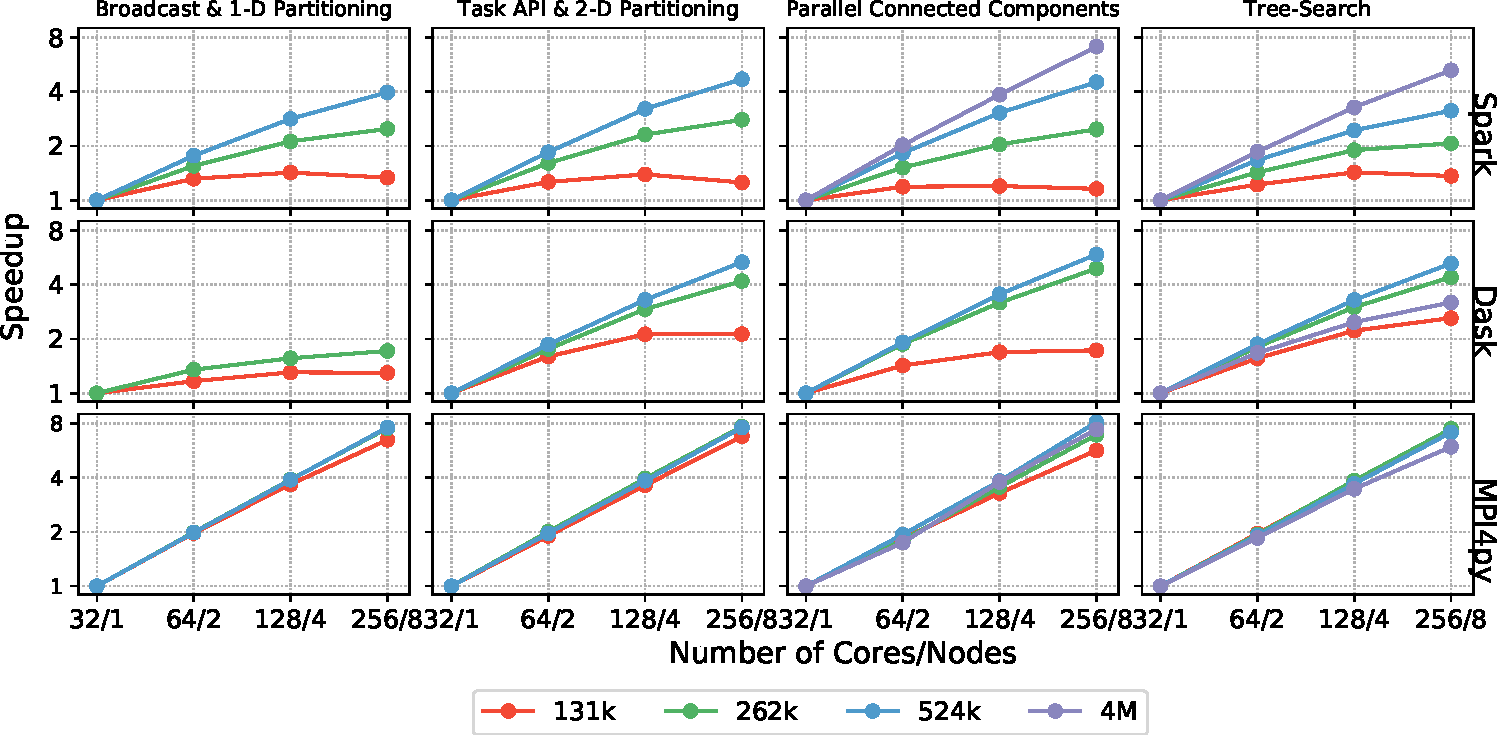
\includegraphics[width=.95\textwidth]{figures/All4approachesWith4MSpeedup.pdf}
        \caption{}
        \label{fig:leafletfinder}
    \end{subfigure}%
    ~ 
    \begin{subfigure}[b]{0.45\textwidth}
        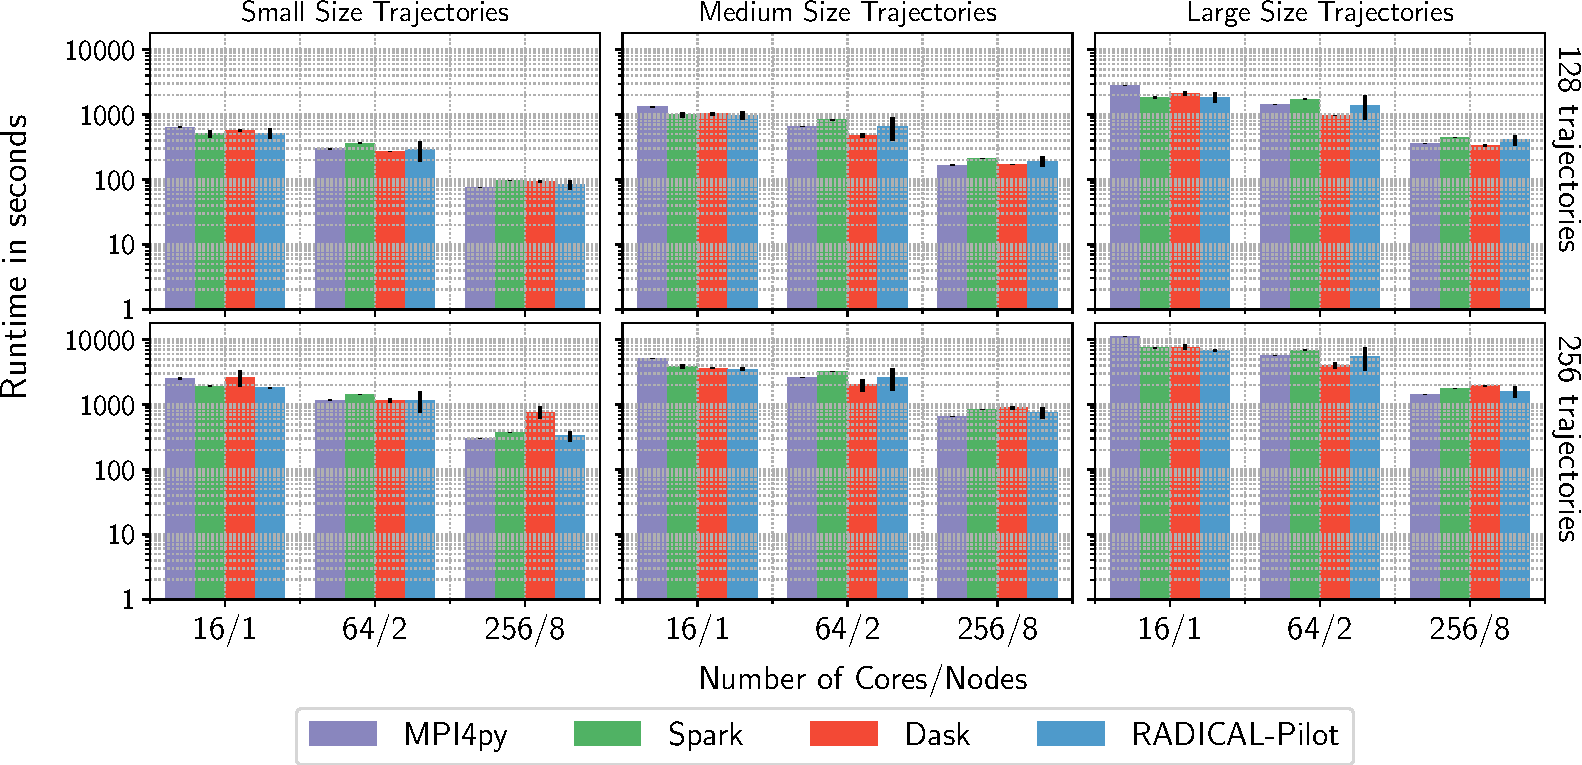
\includegraphics[width=\linewidth]{figures/HausdorffSingleFig.pdf}
        \caption{}
        \label{fig:hausdorff}
    \end{subfigure}
    \caption{Selected molecular dynamics analysis MapReduce algorithm speedup 
    for different frameworks and implementation candidates}\label{fig:md_analysis}
\end{figure*}

As shown in Figure~\ref{fig:leafletfinder}, there are cases where the performance of a parallel implementation is far from ideal, while under different circumstances is as expected. 
For example in Figure~\ref{fig:leafletfinder}, we see that, based on data size Dask provides better speedup than Spark. 
In these cases Dask better utilized the resources compared to Dask, while on others Spark was better.

Implementation aspects, such as computational complexity, and shuffled data size influence the performance greatly. 
For embarrassingly parallel applications with coarse grained tasks the choice of the framework does not significantly influence performance. 
For fine-grained data parallelism, a data-parallel framework is more suited compared to a workload execution framework. 
In addition, the data shuffling size significantly impacts performance and needs to be included in a decision.
The performance analysis of these algorithms implemented in all three frameworks provided us with information to create a conceptual model for selecting the better suitable framework based on algorithmic characteristics.

Data analysis during scientific campaigns may vary depending on the stage of the campaign. 
As a result, the ability to select the best suited framework, given requirements and constraints to execute it is important. 

\subsection{Workflow execution based on middleware design}
\label{design_comp}
Workflow execution time modeling and estimation requires a methodology of 
modeling the execution time of the individual tasks of the workflow as well as 
the overheads imposed by the used middleware. As described in \S2, a task is a 
stand alone process with well defined input, output, termination criteria and 
resource requirements. Classical analysis requires to derive the complexity of 
the algorithm used either analytically or experimentally. The complexity 
function would then provide a model of the execution time of a task. That 
requires that the task's algorithm, as well as its implementation, are well 
known. 

Individual task performance on an HPC resource depends on several factors that 
are not tunable or accessible to the user, such as shared filesystem 
performance, power management policies, and selected runtime system amongst 
others. As a result, the execution time of a task may differ significantly 
between different executions. This breaks from the expectation that a complexity 
based model can provide an accurate estimate. In addition, data intensive tasks 
are highly dependent to the filesystem performance. Thus, we model the 
execution time of a task by considering the tasks as a black box. The only 
information we have prior to execution is the input of the task, for example 
input data size or other parameters.
\gpnote{Can we model the execution time of a task as a distribution whose 
expected value is modeled by the complexity of the algorithm? Makes sense and 
it might include information of }

In Ref.~\cite{paraskevakos2019workflow}, we model the execution time of a 
data-intensive workflow as a function of their input data. Our proposed 
methodology uses a linear function to model the execution time. We fitted the 
function to the data by employing a non-linear least squares algorithm and used 
$R^{2}$ and the error of the estimation as the metrics to validate our fit. 
Specifically, the workflow under investigation requires the execution of two 
tasks consecutively over a set of inputs. The tasks, $T_{1}$ and $T_{2}$, are 
heterogeneous, and have different computational requirements. 
Figure~\ref{fig:sealfitting} shows results of the fitting. In addition, based 
on the $R^{2}$ and standard error values we were able to conclude that our 
fitting produced models that explained the execution time of the tasks.

\begin{figure*}[ht!]
    \centering
    \begin{subfigure}[b]{0.45\textwidth}
        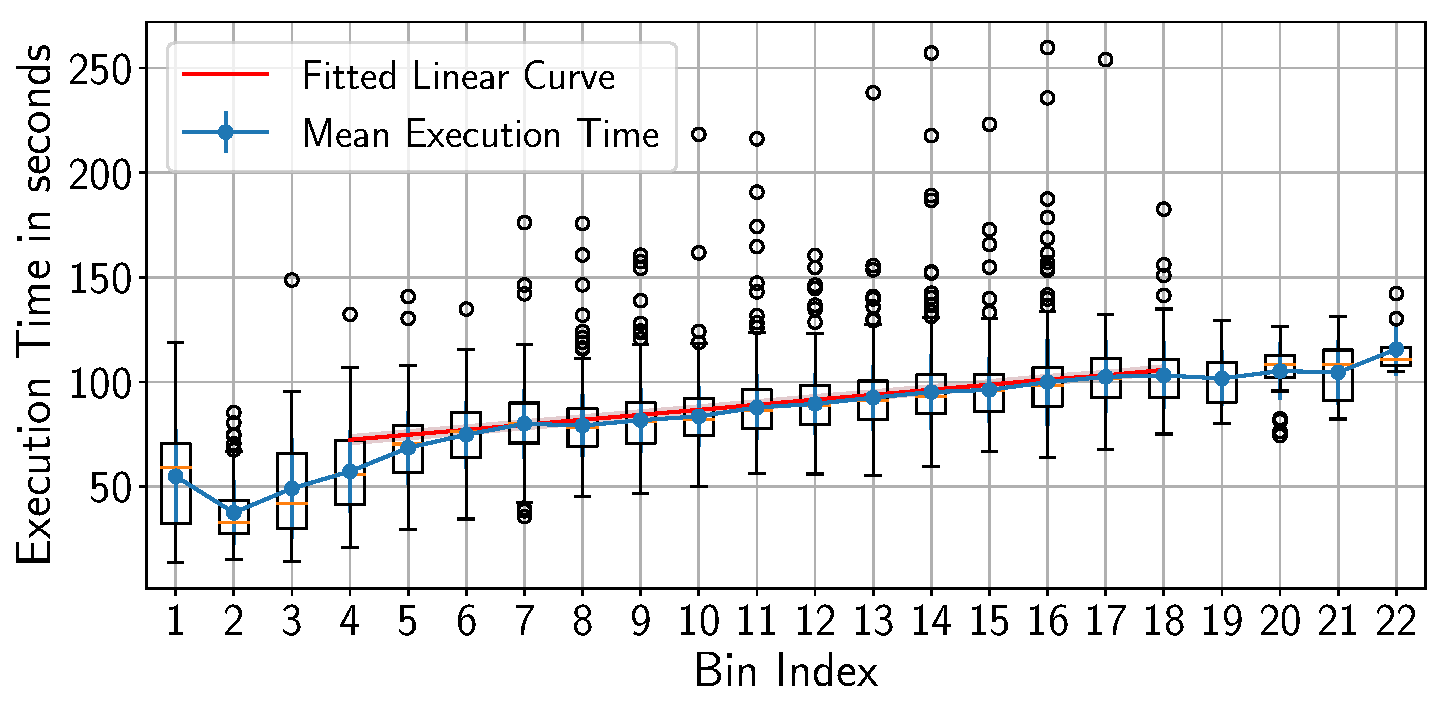
\includegraphics[width=\linewidth]{figures/stage_0_tx_box.pdf}
        \caption{Box-plots of T1 execution time, mean and STD for 125 MB image 
        size bins. Red line shows fitted linear function.}
    \end{subfigure}%
    ~ 
    \begin{subfigure}[b]{0.45\textwidth}
        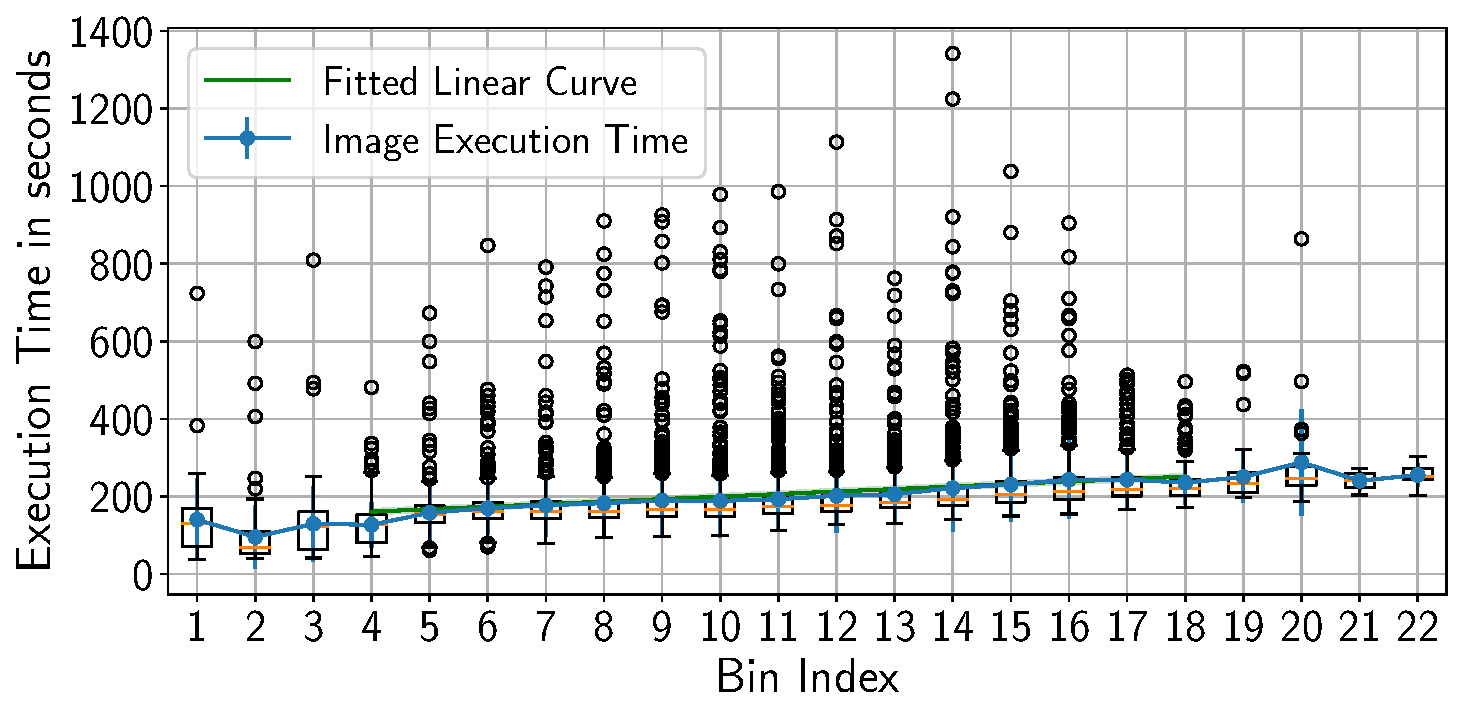
\includegraphics[width=\linewidth]{figures/stage_1_tx_box.pdf}
        \caption{Box-plots of T2 execution time, mean and STD for 125 MB image 
        size bins. Green line shows fitted linear function.}
    \end{subfigure}
    \caption{Task execution time of the tasks of a simple workflow supporting an 
    earth science use case.}
    \label{fig:sealfitting}
\end{figure*}

This works allows us to conclude that modeling the execution time of a task 
based on the initial input, with no knowledge of the specifics, provides an 
accurate estimate. This, in turn can be used to build models for the execution 
of the workflow partitions that comprise the campaign.

\subsection{Related Work}
% ----------------------------------------------------------------------------
% Campaign management system
\gpnote{write about Panda, Blasam, Pegasus, ASKALON, DIRAC, QCFractal(?), GlideInWMS}

There are software systems that are supporting computational campaigns in one way or another. 
PanDA WMS~\cite{maeno2008panda,maeno2014evolution}, possibly the most widely used workload and workflow management system, and DIRAC~\cite{casajus2010dirac}, and glideinWMS~\cite{sfiligoi2008glidein} support domain specific workflows.
These systems assume a specific software stack environment that support their use case.
Our approach is domain agnostic and it makes zero assumptions of a specific pre-existing software stack. 
Furthermore, PanDA, DIRAC, and glideIN are grid oriented campaign managers, without or minimal support of HPC resources.
For example, PanDA undergoes an effort to support HPC~\cite{de2016accelerating}, but it is limited to ORNL Titan~\cite{titan}.
Workflow management systems on HPCs, like Pegasus~\cite{deelman2015pegasus}, and Balsam~\cite{salim2019balsam} support the execution of multiple workflows on HPC resources from multiple users as independent entities.
A common denominator between all the above campaign, workflow or workload managers, is that they provide a capability to define a set of workflows with a common computational objective.
We want to extend this notion and allow users to define a single computational objective for a campaign.
As a result, the above execution model becomes a special case, where a campaign is a single workflow.